\chapter{PREESM}
\label{chapter:preesm}
In this chapter the PREESM rapid prototyping framework is introduced. First an
overview of the framework is given. Second Dataflow models of computation are
discussed. Third development using the PREESM framework is discussed.

\section{PREESM Overview}
\label{sec:preesmover}
The PREESM rapid prototyping framework for multicore development was used to
create a workload application for the thesis experiment \ref{firstexperiment}.
PREESM applications are built using dataflow models. PREESM provides graphical
tools for editing the dataflow diagram and it generates multicore code that is
guaranteed to be deadlock free \cite{pelcat2014preesm}. The code generation can
be configured through graphical tools which provide hints to the scheduler about
the execution time of different actors and rules on which cores they can be
executed on. A PREESM dataflow diagram is presented in figure

\begin{figure}[h!] \label{preesm_example} \begin{center}
    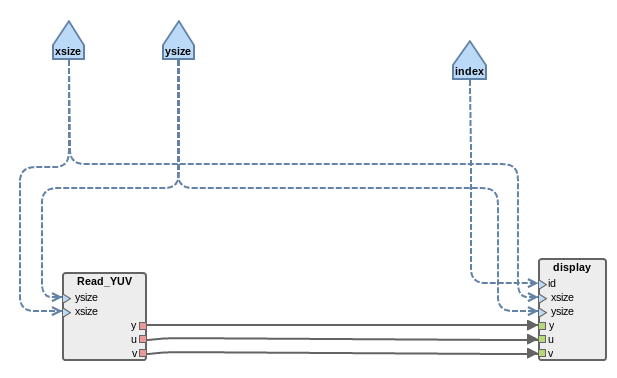
\includegraphics[width=0.99\textwidth]{images/example_preesm_diagram.png}
    \caption{Dataflow diagram used by PREESM} \end{center}
\end{figure}
The reason PREESM was used in the experiment was the need for a simple way to
create multicore applications to provide a baseline for the OpenEM application.

\section{Dataflow Models of Computation}
\label{sec:dataflow}

\section{Development with PREESM}
\label{sec:preesmdev}
